% Auto-generated by 04_additional_analysis.R — do not edit
% y > 0: Underreacts  |  y < 0: Overreacts
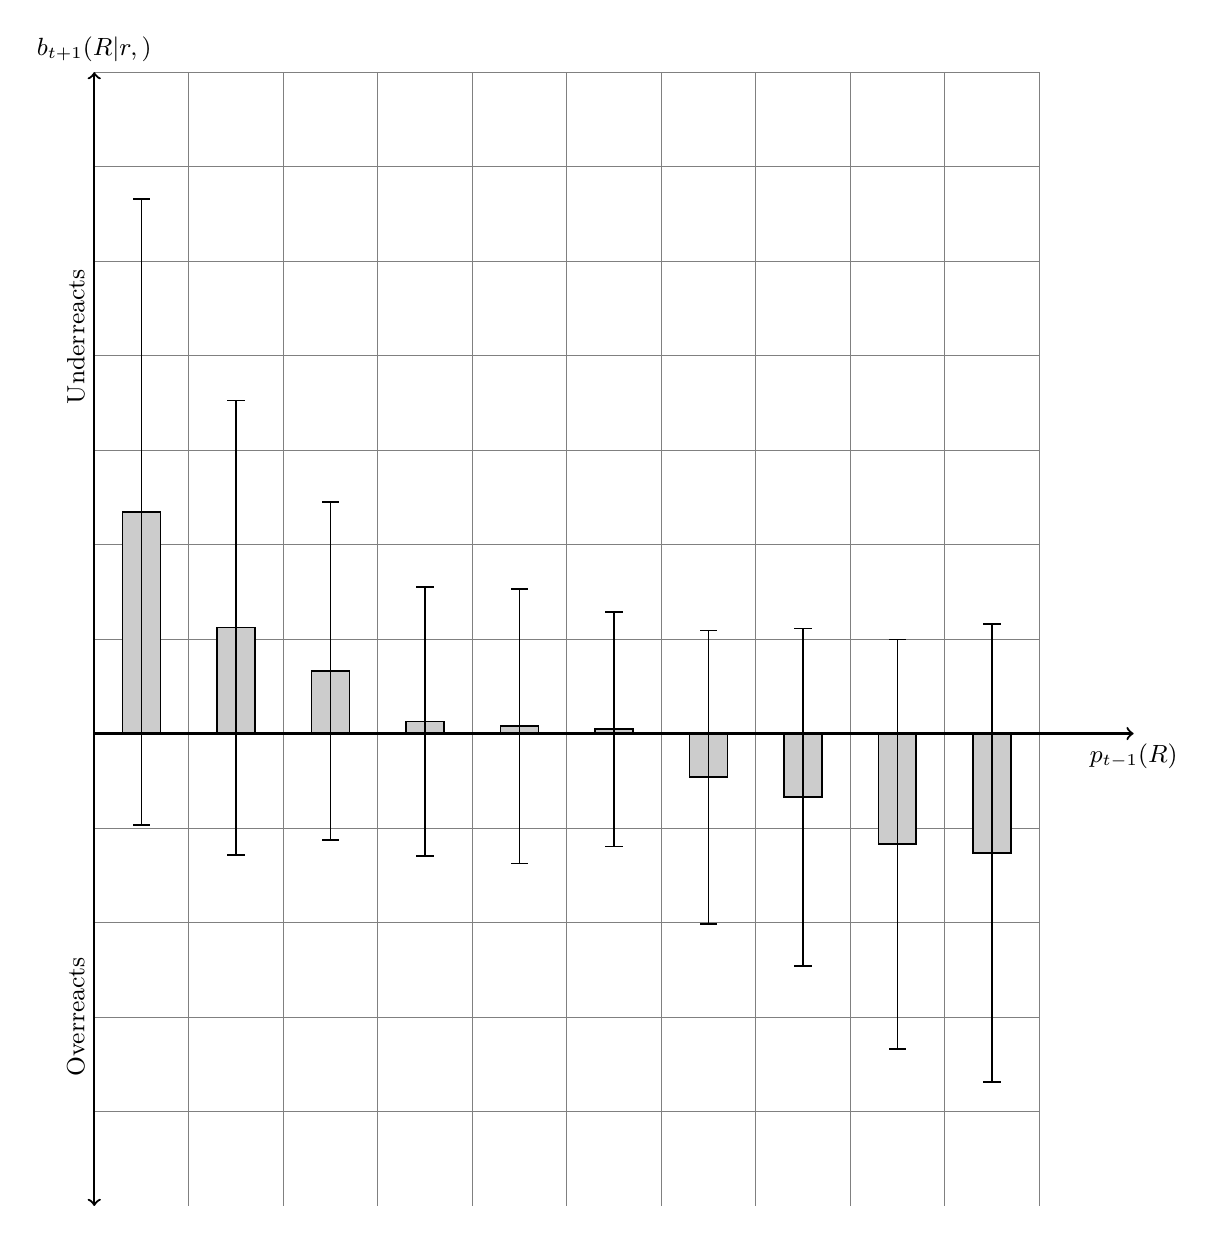
\begin{tikzpicture}[scale=12]
\draw[help lines,step=0.1] (0,-0.5) grid (1,0.7);
\filldraw[opaque,white!80!black] (0.03,0) rectangle (0.07,0.2345);
\draw[line width=0.6] (0.03,0) rectangle (0.07,0.2345);
\draw[line width=0.6,|-|] (0.05,-0.0976) -- (0.05,0.5665);
\filldraw[opaque,white!80!black] (0.13,0) rectangle (0.17,0.1122);
\draw[line width=0.6] (0.13,0) rectangle (0.17,0.1122);
\draw[line width=0.6,|-|] (0.15,-0.1291) -- (0.15,0.3535);
\filldraw[opaque,white!80!black] (0.23,0) rectangle (0.27,0.0661);
\draw[line width=0.6] (0.23,0) rectangle (0.27,0.0661);
\draw[line width=0.6,|-|] (0.25,-0.1136) -- (0.25,0.2457);
\filldraw[opaque,white!80!black] (0.33,0) rectangle (0.37,0.0126);
\draw[line width=0.6] (0.33,0) rectangle (0.37,0.0126);
\draw[line width=0.6,|-|] (0.35,-0.1307) -- (0.35,0.1559);
\filldraw[opaque,white!80!black] (0.43,0) rectangle (0.47,0.0077);
\draw[line width=0.6] (0.43,0) rectangle (0.47,0.0077);
\draw[line width=0.6,|-|] (0.45,-0.1384) -- (0.45,0.1538);
\filldraw[opaque,white!80!black] (0.53,0) rectangle (0.57,0.0048);
\draw[line width=0.6] (0.53,0) rectangle (0.57,0.0048);
\draw[line width=0.6,|-|] (0.55,-0.1203) -- (0.55,0.1298);
\filldraw[opaque,white!80!black] (0.63,0) rectangle (0.67,-0.0461);
\draw[line width=0.6] (0.63,0) rectangle (0.67,-0.0461);
\draw[line width=0.6,|-|] (0.65,-0.2023) -- (0.65,0.1101);
\filldraw[opaque,white!80!black] (0.73,0) rectangle (0.77,-0.0672);
\draw[line width=0.6] (0.73,0) rectangle (0.77,-0.0672);
\draw[line width=0.6,|-|] (0.75,-0.2467) -- (0.75,0.1122);
\filldraw[opaque,white!80!black] (0.83,0) rectangle (0.87,-0.1171);
\draw[line width=0.6] (0.83,0) rectangle (0.87,-0.1171);
\draw[line width=0.6,|-|] (0.85,-0.3346) -- (0.85,0.1004);
\filldraw[opaque,white!80!black] (0.93,0) rectangle (0.97,-0.1265);
\draw[line width=0.6] (0.93,0) rectangle (0.97,-0.1265);
\draw[line width=0.6,|-|] (0.95,-0.3694) -- (0.95,0.1165);
\draw[line width=0.8,->]  (0,0) -- (1.1,0) node[below] {\small{$p_{t-1}(R)$}};
\draw[line width=0.8,<->] (0,-0.5) -- (0,0.7) node[above] {\small{$b_{t+1}(R|r,\xmark)$}};
\draw (0,0.42) node[above,rotate=90] {\small{Underreacts}};
\draw (0,-0.30) node[above,rotate=90] {\small{Overreacts}};
% ADD THEORY CURVE BELOW IF NEEDED:
% \draw[red,line width=1.2,domain=0.01:0.99] plot(\x,{...});
\end{tikzpicture}
